%-----------------------------------------------------------------------
% Beginning of chapter.tex
%-----------------------------------------------------------------------
%
%  This is a sample file for use with AMS-LaTeX.  It provides an example
%  of how to set up a file for a book to be typeset with AMS-LaTeX.
%
%  This is the driver file.  Separate chapters should be included at
%  the end of this file.
%
%  ***** DO NOT USE THIS FILE AS A STARTER FOR YOUR BOOK. *****
%  Follow the guidelines in the file chapter.template.
%
%%%%%%%%%%%%%%%%%%%%%%%%%%%%%%%%%%%%%%%%%%%%%%%%%%%%%%%%%%%%%%%%%%%%%%%%

\documentclass[11pt,a4paper]{memoir}
\chapterstyle{demo}
\epigraphfontsize{\small\itshape}
\setlength\epigraphwidth{8cm}
\setlength\epigraphrule{0pt}
\epigraphfontsize{\small\itshape}
%\includeonly{preface,chap1,biblio}

%\numberwithin{section}{chapter}
%\numberwithin{equation}{chapter}

% Include macros here
%=================================================
% Packages
%=================================================

%\usepackage{fixltx2e}
\usepackage[usenames,dvipsnames]{xcolor}
%\usepackage{fancyhdr}
\usepackage{amsmath,amsfonts,amsbsy,amsgen,amscd,mathrsfs,amssymb,amscd}
\usepackage{amsthm}
\usepackage{bm}
\usepackage{url}
\usepackage[UKenglish]{babel}
\usepackage{eurosym}
\usepackage{tikz}
\usepackage{caption}
\usetikzlibrary{matrix,arrows,shapes,calc,3d}
\usepackage{tikz-3dplot}
\tdplotsetmaincoords{60}{110}
\pgfmathsetmacro{\rvec}{.8}
\pgfmathsetmacro{\thetavec}{30}
\pgfmathsetmacro{\phivec}{60}

\tikzset{mynode/.style = {
    % The shape
    circle,
    % The size
    minimum size=2pt,
    % The color
    draw=black, fill=black}
}
\tikzset{vertex/.style={shape=circle, % style for a vertex
                        minimum size=3pt,
                        fill=gray,
                        inner sep = 0pt}}  

% \usepackage{3dplot}
% \tdplotsetmaincoords{60}{110}
%\usepackage{subfig}
\usepackage{microtype}
\usepackage{enumitem}
\usepackage{listings}
\definecolor{darkblue}{rgb}{0,0,.75}

\usepackage[many]{tcolorbox}
\tcbuselibrary{listings}

\definecolor{light-gray}{rgb}{0.96,0.96,0.96}
\definecolor{kwgreen}{rgb}{0,0.5,0}
\definecolor{cogreen}{rgb}{0.25,0.5,0.5}
\definecolor{mygreen}{rgb}{0,0.5,0.125}
\definecolor{equalsign}{rgb}{0.66,0.13,1}
\definecolor{darkred}{rgb}{0.75,0.16,0.37}

\lstloadlanguages{Python} %use listings with Python
%\lstset{literate={==}{{\color{equalsign}==}} {\*}{{\color{equalsign}\*}}}
%\lstnewenvironment{PseudoCode}[1][]
% the space reserved between for the ``In'' numbers and the code
\newlength\inwd
\setlength\inwd{1.7cm}

\newcounter{ipythcntr}

\newtcblisting{ipythonnb}[1][\theipythcntr]{
  enlarge left by=\inwd,
  width=\linewidth-\inwd,
  enhanced,
  boxrule=0.4pt,
  boxsep=0pt,
  left=2pt,
  top=0pt,
  colback=light-gray,
  listing only,
  top=0pt,
  bottom=0pt,
  arc=1pt,
  overlay={
    \node[
      anchor=north east,
      text width=\inwd,
      font=\footnotesize\ttfamily\color{blue!50!black},
      inner ysep=2.5mm,
      inner xsep=0pt,
      outer sep=0pt
      ] 
      at (frame.north west)
      {\stepcounter{ipythcntr}In [#1]:};
  }
  listing style=Python,
  listing options={
    basicstyle=\scriptsize\ttfamily\color{black},
    language=Python,
    escapechar=£,
    showstringspaces=false,
    commentstyle=\color{cogreen},
    keywordstyle=\bfseries\color{kwgreen},
    stringstyle=\color{darkred},
    numberstyle=\color{kwgreen},
    identifierstyle=\color{black},
    %emph={from,import,as},          % Custom highlighting
    otherkeywords={0,1,2,3,4,5,6,7,8,9,\*,==,<=,>=,+,-,\%},
    emph={*,==,<=,>=,+,-,\%},    
    emphstyle=\color{equalsign},
    extendedchars=true,
  },
}

\newtcblisting{ipythonnbout}[1][\theipythcntr]{
  enlarge left by=\inwd,
  width=\linewidth-\inwd,
  enhanced,
  boxrule=0pt,
  boxsep=0pt,
  left=2pt,
  top=0pt,
  colback=white,
  listing only,
  top=0pt,
  bottom=0pt,
  frame hidden,
  overlay={
    \node[
      anchor=north east,
      text width=\inwd,
      font=\footnotesize\ttfamily\color{red},
      inner ysep=2.5mm,
      inner xsep=0pt,
      outer sep=0pt
      ] 
      at (frame.north west)
      {\stepcounter{ipythcntr}Out [#1]:};
  }
  listing style=Python,
  listing options={
    basicstyle=\scriptsize\ttfamily\color{black},
    language=Python,
    escapechar=£,
    showstringspaces=false,
    commentstyle=\color{cogreen},
    keywordstyle=\bfseries\color{kwgreen},
    stringstyle=\color{darkred},
    numberstyle=\color{kwgreen},
    identifierstyle=\color{black},
    %emph={from,import,as},          % Custom highlighting
%    otherkeywords={as,0,1,2,3,4,5,6,7,8,9,\*,==,<=,>=,+,-},
%    emph={*,==,<=,>=,+,-},    
%    emphstyle=\color{equalsign},
    extendedchars=true,
    %literate={#}{{\#}},
  },
}

\newtcblisting{ipythonnboutno}{
  enlarge left by=\inwd,
  width=\linewidth-\inwd,
  enhanced,
  boxrule=0pt,
  boxsep=0pt,
  left=2pt,
  top=0pt,
  colback=white,
  listing only,
  top=0pt,
  bottom=0pt,
  frame hidden,
  overlay={
    \node[
      anchor=north east,
      text width=\inwd,
      font=\footnotesize\ttfamily\color{red},
      inner ysep=2.5mm,
      inner xsep=0pt,
      outer sep=0pt
      ] 
      at (frame.north west)
      {};
  }
  listing style=Python,
  listing options={
    basicstyle=\scriptsize\ttfamily\color{black},
    language=Python,
    escapechar=£,
    showstringspaces=false,
    commentstyle=\color{cogreen},
    %keywordstyle=\bfseries\color{kwgreen},
    stringstyle=\color{darkred},
    numberstyle=\color{kwgreen},
    identifierstyle=\color{black},
    %emph={from,import,as},          % Custom highlighting
    %otherkeywords={as,0,1,2,3,4,5,6,7,8,9,\[,\]},
    %emph={[,]},    
    %emphstyle=\color{black},
    extendedchars=true,
    %literate={#}{{\#}},
  },
}


%{\lstset{language=Matlab,basicstyle=\small, keywordstyle=\color{darkblue},numbers=none,xleftmargin=.04\textwidth,mathescape,frame=single,#1}}
%{}
%\usepackage[]{algorithm2e}
%\usepackage{mcode}
\usepackage{multicol}

%\usepackage[draft]{changes}
%\definechangesauthor[color=blue]{ml}
%\definechangesauthor[color=red]{da}
% \usepackage{trackchanges}
% \addeditor{ml}
% \addeditor{da}

\definecolor{dark-gray}{gray}{0.3}
\definecolor{dkgray}{rgb}{.4,.4,.4}
\definecolor{dkblue}{rgb}{0,0,.5}
\definecolor{medblue}{rgb}{0,0,.75}
\definecolor{rust}{rgb}{0.5,0.1,0.1}

\usepackage[colorlinks=true]{hyperref}
\hypersetup{urlcolor=Blue}
\hypersetup{citecolor=Black}
\hypersetup{linkcolor=dark-gray}

%\usepackage{setspace}
\usepackage{graphicx}
%\usepackage{multicol}
\usepackage{booktabs,longtable,tabu} % Nice tables
\setlength{\tabulinesep}{1pt}
\usepackage{multirow} % More control over tables
\usepackage{float}
\usepackage[T1]{fontenc}
%\usepackage{quotchap}

% Fonts
\usepackage{times}
%\usepackage{fourier}
%\usepackage[no-math]{fontspec}
%\setmainfont{optima}
%\usepackage{charter}
\usepackage{bm} % boldmath must be called after the package

%=================================================
% Paths
%=================================================

\graphicspath{{figures/}}

%=================================================
% Formatting
%=================================================

%\sloppy % Helps with margin justification

%%% Further font changes
\newcommand{\lang}{\textit}
\newcommand{\titl}{\textsl}
\newcommand{\term}{\emph}

%%% Equation numbering
\numberwithin{equation}{section} 

%%% Typesetting
\providecommand{\mathbold}[1]{\bm{#1}}  % Must be after 'fourier'
                                % package loads
%%% Annotations
\newcommand{\notate}[1]{\textcolor{red}{\textbf{[#1]}}}

%=================================================
% Theorem environment
%=================================================

\newtheorem{bigthm}{Theorem}
\renewcommand{\thebigthm}{\Roman{bigthm}}

\newtheorem{theorem}{Theorem}[section]
\newtheorem{lemma}[theorem]{Lemma}
\newtheorem{sublemma}[theorem]{Sublemma}
\newtheorem{proposition}[theorem]{Proposition}
\newtheorem{fact}[theorem]{Fact}
\newtheorem{result}[theorem]{Result}
\newtheorem{conjecture}[theorem]{Conjecture}
\newtheorem{corollary}[theorem]{Corollary}

\newtheorem{problem}[theorem]{Problem}
\newtheorem{solution}[theorem]{Solution}

\theoremstyle{definition}

\newtheorem{definition}[theorem]{Definition}
\newtheorem{example}[theorem]{Example}
\newtheorem{remark}[theorem]{Remark}

\newenvironment{mainthm}{\par\textsc{Main theorem.}\it}{\par}
\renewcommand{\thebigthm}{\Alph{bigthm}}

%=================================================
% Symbols
%=================================================

%%% Old symbols with new names
\newcommand{\oldphi}{\phi}
\renewcommand{\phi}{\varphi}

\newcommand{\eps}{\varepsilon}
\newcommand{\e}{\varepsilon}

%\newcommand{\oldmid}{\mid}
\renewcommand{\mid}{\mathrel{\mathop{:}}} 

%%% New symbols
\newcommand{\defby}{\overset{\mathrm{\scriptscriptstyle{def}}}{=}}
\newcommand{\half}{\tfrac{1}{2}}
\newcommand{\third}{\tfrac{1}{3}}

\newcommand{\sumnl}{\sum\nolimits}

\newcommand{\defeq}{\ensuremath{\mathrel{\mathop{:}}=}} % Definition-equals
\newcommand{\eqdef}{\ensuremath{=\mathrel{\mathop{:}}}} % Equals-definition

%%% Constants
\newcommand{\cnst}[1]{\mathrm{#1}} 
\newcommand{\econst}{\mathrm{e}}
\newcommand{\iunit}{\mathrm{i}}

\newcommand{\onevct}{\mathbf{e}} % All ones vector
\newcommand{\zerovct}{\vct{0}} % Zero vector

\newcommand{\Id}{\mathbf{I}}
\newcommand{\onemtx}{\bm{1}}
\newcommand{\zeromtx}{\bm{0}}

%%% Sets
\newcommand{\coll}[1]{\mathscr{#1}}
\newcommand{\sphere}[1]{S^{#1}}
\newcommand{\ball}[1]{B^{#1}}
\newcommand{\Grass}[2]{\mathbb{G}(#1,#2)}
\providecommand{\mathbbm}{\mathbb} % In case we don't load bbm
\newcommand{\Rplus}{\mathbbm{R}_{+}}
\newcommand{\R}{\mathbbm{R}}
\newcommand{\C}{\mathbbm{C}}
\newcommand{\N}{\mathbbm{N}}
\newcommand{\FF}{\mathbbm{F}}
\newcommand{\struct}{\mathcal{S}}

% Group theory
\newcommand{\stab}{\mathrm{stab}}

% Algebra
\newcommand{\End}{\mathrm{End}}
\newcommand{\Hom}{\mathrm{Hom}}
\newcommand{\Mult}{\mathrm{Mult}}

% Set operations
\newcommand{\polar}{\circ}
\newcommand{\closure}{\overline}
\newcommand{\prtensor}{\,\hat{\otimes}\,}

%%% Real and complex analysis
\newcommand{\abs}[1]{\left\vert {#1} \right\vert}
\newcommand{\abssq}[1]{{\abs{#1}}^2}

\newcommand{\sgn}[1]{\operatorname{sgn}{#1}}
\newcommand{\real}{\operatorname{Re}}
\newcommand{\imag}{\operatorname{Im}}
\newcommand{\pos}{\operatorname{Pos}}
\newcommand{\shrink}{\operatorname{Shrink}}

\newcommand{\diff}[1]{\mathrm{d}{#1}}
\newcommand{\idiff}[1]{\, \diff{#1}}

\newcommand{\gradd}{\mathrm{grad }} % Conflicts w/SIAM styles?
\newcommand{\divv}{\mathrm{div }}
\newcommand{\subdiff}{\partial}

%%% Optimization

\newcommand{\minimize}{\text{minimize}\quad}
\newcommand{\maximize}{\text{maximize}\quad}
\newcommand{\subjto}{\quad\text{subject to}\quad}
\newcommand{\find}{\text{find}\quad}
\newcommand{\suchthat}{\quad\text{such that}\quad}

\newcommand{\argmin}{\operatorname*{arg\; min}}
\newcommand{\argmax}{\operatorname*{arg\; max}}
\newcommand{\dom}{\mathrm{dom} }

%%% Probability & measure

\newcommand{\Prob}{\mathbbm{P}}
\newcommand{\Probe}[1]{\Prob\left({#1}\right)}
\newcommand{\Expect}{\operatorname{\mathbb{E}}}

\newcommand{\St}{\operatorname{St}}

%\newcommand{\normal}{\textsc{Normal}}
\newcommand{\normal}{N}
\newcommand{\uniform}{\textsc{Uniform}}
\newcommand{\erf}{\operatorname{erf}}

\DeclareMathOperator{\rvol}{rvol}
\DeclareMathOperator{\Var}{Var}
\DeclareMathOperator{\Gl}{Gl}
\newcommand{\diag}{\operatorname{diag}}

%%% Vector and matrix operators
\newcommand{\vct}[1]{\mathbold{#1}}
\newcommand{\mtx}[1]{\mathbold{#1}}
\newcommand{\Eye}{\mathbf{I}}

\newcommand{\transp}[1]{#1^{T}}
\newcommand{\trans}{\top}
\newcommand{\adj}{*}
\newcommand{\psinv}{\dagger}

\newcommand{\lspan}[1]{\operatorname{span}{#1}}

\newcommand{\range}{\operatorname{range}}
\newcommand{\colspan}{\operatorname{colspan}}

%\newcommand{\rank}{\operatorname{rank}}
\newcommand{\nullity}{\operatorname{null}}
%\newcommand{\ker}{\operatorname{ker}}
\newcommand{\im}{\operatorname{im}}
%\newcommand{\span}{\operatorname{span}}

%\newcommand{\diag}{\operatorname{diag}}
\newcommand{\trace}{\operatorname{tr}}

\newcommand{\supp}[1]{\operatorname{supp}(#1)}
\newcommand{\sign}[1]{\operatorname{sign}(#1)}

\newcommand{\smax}{\sigma_{\max}}
\newcommand{\smin}{\sigma_{\min}}

\newcommand{\nnz}{\operatorname{nnz}}
\renewcommand{\vec}{\operatorname{vec}}

\newcommand{\Proj}{\ensuremath{\mtx{\Pi}}} % Projection operator

%%% Semidefinite orders
\newcommand{\psdle}{\preccurlyeq}
\newcommand{\psdge}{\succcurlyeq}

\newcommand{\psdlt}{\prec}
\newcommand{\psdgt}{\succ}

%%% Mensuration: inner products and norms

% TeX does not like either \newcommand or \renewcommand for these
% two macros.  There is probably a good reason not to use them via
% \def, but I don't know it.  
%\newcommand{\<}{\langle} 
%\newcommand{\>}{\rangle}
\newcommand{\ip}[2]{\langle {#1}, {#2} \rangle}
% --deleted the \left and \right-- Dennis
% \newcommand{\ip}[2]{\left\langle {#1},\ {#2} \right\rangle}
\newcommand{\absip}[2]{\abs{\ip{#1}{#2}}}
\newcommand{\abssqip}[2]{\abssq{\ip{#1}{#2}}}
\newcommand{\tworealip}[2]{2 \, \real{\ip{#1}{#2}}}

%\newcommand{\norm}[1]{\left\Vert {#1} \right\Vert}
\newcommand{\norm}[1]{\Vert {#1}\Vert}
\newcommand{\normsq}[1]{\norm{#1}^2}

\newcommand{\lone}[1]{\norm{#1}_{\ell_1}}
\newcommand{\smlone}[1]{\|#1\|_{\ell_1}}
\newcommand{\linf}[1]{\norm{#1}_{\ell_\infty}}
\newcommand{\sone}[1]{\norm{#1}_{S_1}}
\newcommand{\snorm}[1]{\sone{#1}}
\newcommand{\wnnorm}[1]{\norm{#1}_{*,\vct{w}}}
\newcommand{\wnnormd}[1]{\norm{#1}^*_{\vct{w}}}
\DeclareMathOperator{\dist}{dist}

% Fixed-size inner products and norms are useful sometimes
\newcommand{\smip}[2]{\bigl\langle {#1}, \ {#2} \bigr\rangle}
\newcommand{\smabsip}[2]{\bigl\vert \smip{#1}{#2} \bigr\vert}
\newcommand{\smnorm}[2]{{\bigl\Vert {#2} \bigr\Vert}_{#1}}

% Specific norms that are used frequently
\newcommand{\enormdangle}{{\ell_2}}
\newcommand{\enorm}[1]{\norm{#1}}
\newcommand{\enormsm}[1]{\enorm{\smash{#1}}}

\newcommand{\enormsq}[1]{\enorm{#1}^2}

\newcommand{\fnorm}[1]{\norm{#1}_{\mathrm{F}}}
\newcommand{\fnormsq}[1]{\fnorm{#1}^2}

\newcommand{\pnorm}[2]{\norm{#2}_{#1}}
%\newcommand{\snorm}[1]{\norm{#1}_*}

\newcommand{\triplenorm}[1]{\left\vert\!\left\vert\!\left\vert {#1} \right\vert\!\right\vert\!\right\vert} 

\newcommand{\flag}[2]{{#1 \brack #2}}

% Special cones
\newcommand{\Feas}{\mathcal{F}}
\newcommand{\Desc}{\mathcal{D}}

\newcommand{\sdim}{\delta}
\newcommand{\sdimw}{\delta^*}
% \newcommand{\sdimw}{\tilde{\delta}}
\newcommand{\ddt}[1]{\dot{#1}}
\DeclareMathOperator{\Circ}{Circ}

%%% Differential geometry
\newcommand{\Cinf}{C^{\infty}}
\newcommand{\Tensf}{\mathcal{T}}
\newcommand{\Vbundle}{\mathcal{X}}
\newcommand{\Christ}[3]{\Gamma_{{#1}{#2}}^{#3}}

% Stuff to be sorted in somewhere
\DeclareMathOperator{\Lip}{Lip}

\newcommand{\IR}{\mathbbm{R}}
\newcommand{\veps}{\varepsilon}
\newcommand{\mA}{\mathcal{A}}
\newcommand{\mB}{\mathcal{B}}
\newcommand{\mC}{\mathcal{C}}
\newcommand{\mD}{\mathcal{D}}
\newcommand{\mE}{\mathcal{E}}
\newcommand{\mI}{\mathcal{I}}
\newcommand{\mM}{\mathcal{M}}
\newcommand{\mN}{\mathcal{N}}
\newcommand{\mL}{\mathcal{L}}
\newcommand{\mV}{\mathcal{V}}
\newcommand{\bface}{\overline{\mathcal{F}}}
\newcommand{\face}{\mathcal{F}}
\newcommand{\relint}{\operatorname{relint}}
\newcommand{\relcl}{\operatorname{relcl}}
\newcommand{\cone}{\operatorname{cone}}
\newcommand{\lin}{\operatorname{lin}}
\newcommand{\Gr}{\operatorname{Gr}}
\newcommand{\powerset}{\mathscr{P}}
\newcommand{\hd}{{\operatorname{hd}}}
\newcommand{\inter}{{\operatorname{int}}}
\newcommand{\conv}{\operatorname{conv}}
\newcommand{\clconv}{\overline{\conv}}
\newcommand{\cl}{\operatorname{cl}}
\newcommand{\bd}{\operatorname{bd}}

\newcommand{\GL}{\operatorname{GL}}

% \newcommand{\tb}{\stackrel{0}{\to}}
\newcommand{\tb}{\,\,\mathring{\to}\,\,}
% \newcommand{\tdash}{\,\,\overset{e}{\to}\,\,}
% \newcommand{\tdash}{\,\,\overset{a}{\to}\,\,}
\newcommand{\tdash}{\overset{a}{\to}}

\newcommand{\K}{\mathcal{K}}
\newcommand{\B}{\mathcal{B}}
\newcommand{\F}{\mathcal{F}}
\newcommand{\D}{\mathcal{D}}
\renewcommand{\P}{\mathcal{P}}
\DeclareMathOperator{\id}{id}
\DeclareMathOperator{\gr}{gr}
\newcommand{\vp}{\varphi}
\newcommand{\maxp}{{\max}_p}
\DeclareMathOperator{\spa}{span}
\DeclareMathOperator{\vol}{vol}
\DeclareMathOperator{\ima}{im}
\DeclareMathOperator{\rk}{rk}

\newcommand{\Ren}{\mathcal{R}}
\newcommand{\T}{\mathcal{T}}
% ADJUST THE FOLLOWING
% \newcommand{\resTMP}[2]{#1,#2}
\newcommand{\resTMP}[2]{#1\to#2}
% 
\newcommand{\res}[3]{\vct{#1}_{\resTMP{#2}{#3}}}
\newcommand{\nres}[3]{\|\vct{#1}\|_{\resTMP{#2}{#3}}}
\newcommand{\sres}[3]{\sigma_{\resTMP{#2}{#3}}(\vct{#1})}
\newcommand{\csres}[3]{\overline{\sigma}_{\resTMP{#2}{#3}}(\vct{#1})}
\newcommand{\kres}[3]{\kappa_{\resTMP{#2}{#3}}(\vct{#1})}
% transpose
\newcommand{\rest}[3]{\vct{#1}^T_{\resTMP{#2}{#3}}}
\newcommand{\nrest}[3]{\|\vct{#1}^T\|_{\resTMP{#2}{#3}}}
\newcommand{\srest}[3]{\sigma_{\resTMP{#2}{#3}}(\vct{#1}^T)}
\newcommand{\csrest}[3]{\overline{\sigma}_{\resTMP{#2}{#3}}(\vct{#1}^T)}
\newcommand{\srestm}[3]{\sigma_{\resTMP{#2}{#3}}(-\vct{#1}^T)}
\newcommand{\krest}[3]{\kappa_{\resTMP{#2}{#3}}(\vct{#1}^T)}
\newcommand{\nresdag}[3]{\|\vct{#1}^\dagger\|_{\resTMP{#2}{#3}}}

\newcommand{\RCD}[3]{\Ren_{#2,#3}(\vct{#1})}
% \newcommand{\RCD}[3]{\Ren_{\resTMP{#2}{#3}}(\vct{#1})}

\newcommand{\DA}{\vct{\Delta A}}

%
\newcommand{\Rmm}{R_{\mathrm{mm}}}

\newcommand{\rbinom}[2]{\genfrac{[}{]}{0pt}{}{#1}{#2}}
\newcommand{\trbinom}[2]{{\textstyle\genfrac{[}{]}{0pt}{}{#1}{#2}}}

\newcommand{\comm}[1]{\textcolor{red}{\textbf{[#1]}}}
\newcommand{\rant}[1]{\textcolor{blue}{\textbf{[#1]}}}
%

\newcommand{\llangle}{\langle\hspace{-1.5pt}\langle}  % this is actually contained in mnsymbol, but loading this package causes trouble...
\newcommand{\rrangle}{\rangle\hspace{-1.5pt}\rangle}  % this is actually contained in mnsymbol, but loading this package causes trouble...

\newcommand{\Res}{\mathrm{Res}}
\newcommand{\Oh}{\mathcal{O}}
\newcommand{\Mbar}{\overline{M}}
\newcommand{\second}{\mathrm{II}}
\newcommand{\nablabar}{\overline{\nabla}}
\newcommand{\expm}{\mathrm{exp}}
\newcommand{\Rc}{\mathrm{Rc}}
\newcommand{\NJ}{\mathrm{NJ}}
% %\newcommand{\GL}[1]{\mathrm{GL}(#1)}

\newcommand{\cover}{\lessdot}

% Semidefinite programming
\newcommand{\Sym}{\mathcal{S}}
\newcommand{\SDP}{\mathcal{S}_+}
\newcommand{\psd}{\succeq}
\newcommand{\bdot}{\bullet}

%\renewcommand{\chaptername}{}
%\renewcommand{\thechapter}{}

\begin{document}
%\numberwithin{section}{chapter}
\numberwithin{equation}{chapter}
\numberwithin{theorem}{chapter}

\lstset{language=Matlab}

%\frontmatter
%\title{Convex Optimization}

%    Information for first author
%\author{Martin Lotz}
%    Address of record for the research reported here

%\address{School of Mathematics\\ The University of Manchester\\ Alan Turing Building, Oxford Road\\ Manchester M139PL}

%\email{martin.lotz@manchester.ed.uk}
%\urladdr{http://www.maths.manchester.ac.uk/\textasciitilde mlotz}

%\date{\today}

%\maketitle

%\newpage 

%\tableofcontents

%\include{preface}

\mainmatter

%\include{notation}
%-----------------------------------------------------------------------
% Beginning of chap2.tex
%-----------------------------------------------------------------------
%
%  AMS-LaTeX sample file for a chapter of a monograph, to be used with
%  an AMS monograph document class.  This is a data file input by
%  chapter.tex.
%
%  Use this file as a model for a chapter; DO NOT START BY removing its
%  contents and filling in your own text.
% 
%%%%%%%%%%%%%%%%%%%%%%%%%%%%%%%%%%%%%%%%%%%%%%%%%%%%%%%%%%%%%%%%%%%%%%%%


\chapter*{Lecture 14}
\addcontentsline{toc}{chapter}{Lecture 14}
\addtocounter{chapter}{14}
%\addtocounter{section}{-2}
%\numberwithin{section}{chapter}
\numberwithin{equation}{chapter}
\numberwithin{theorem}{chapter}

%\epigraph{}{--- \textup{}}

So far we have only dealt with constrained optimization problems where the objective and the constraints are linear. We now turn attention to general problems of the form

\begin{align*}\label{eq:constr}\tag{1}
\begin{split}
 \minimize & f(\vct{x})\\
 \subjto & \vct{f}(\vct{x})\leq \zerovct\\
         & \vct{h}(\vct{x})= \zerovct,
\end{split}
\end{align*}
where $\vct{x}\in \R^n$, $\vct{f}=(f_1,\dots,f_m)^{\trans}$, $\vct{h}=(h_1,\dots,h_{p})$, and the inequalities are componentwise. 
The problem~\eqref{eq:constr} is {\em convex}, if $f$ and the $g_i$ are convex, and the $h_j$ are linear. We also denote by $\mathrm{dom}(f)$ the {\em domain} of $f$, which is the set of points $\vct{x}$ where $f$ takes a finite value. The feasible set
\begin{equation*}
 \mathcal{F} = \{\vct{x} \mid f_i(\vct{x})\leq 0, \ h_j(\vct{x})=0, \ 1\leq i\leq m, \ 1\leq j\leq \ell\}
\end{equation*}
for a convex constrained problem is a convex set.

\section{Quadratic Programming and Portfolio Optimization}
The simplest case of non-linear, constrained convex optimization is \textbf{quadratic programming}. Quadratic programming problems are of the form
\begin{align*}
  \minimize & \frac{1}{2}\vct{x}^{\trans}\mtx{Q}\vct{x}+\vct{c}^{\trans}\vct{x}\\
  \subjto & \mtx{A}\vct{x}\leq \vct{b},
\end{align*}
with $\mtx{Q}$ symmetric and positive semidefinite.
Note that this problem combines two problems we studied in some detail before: minimizing a quadratic function, and linear constraints. Just as we did for unconstrained minimization and for linear programming, we will derive optimality conditions for such problems. Before studying the theory, we first present an important application: portfolio optimization.

\subsection{Mean-variance portfolio theory}
If we invest an amount $x^0$ into a product at period $0$, and at period $1$ (for example, one day) the value is $x^1$, then the \textbf{relative return} is defined as
\begin{equation*}
  r = \frac{x^{1}-x^{0}}{x^{0}}.
\end{equation*}

The following figure shows the price movement and the returns of a stock from January 2016 until now.

\begin{figure}
\centering
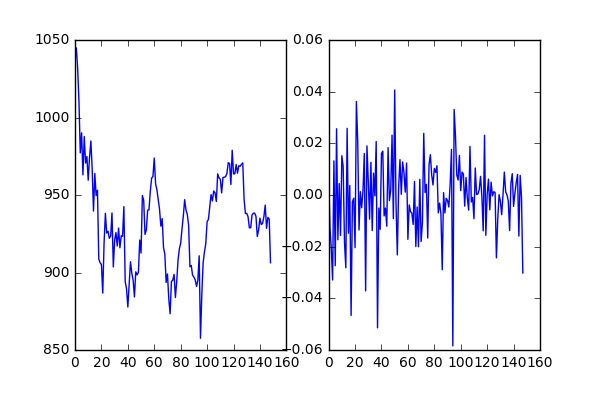
\includegraphics[width=0.8\textwidth]{images/stock.png}
\end{figure}

As we can't predict the future, we usually work with the \textbf{expected return} $\mtx{E}[r]=\mu$, which is a statistical estimate of the future return. One naive method of estimating the future return is by taking the average of past returns, but other more sophisticated methods are possible.

In \textbf{portfolio optimization}, we have a proportion $x_i$ of our available funds that we want to invest in a stock $i$ (in particular, as $x_i$ measures a proportion, we have $\sum_{i=1}^n x_i = 1$). We may or may not allow $x_i<0$, which would correspond to short-selling or borrowing. Given this allocation, the overall return is $\vct{x}^{\trans}\vct{r}$, where $\vct{x}=(x_1,\dots,x_n)^{\trans}$ and $\vct{r}=(r_1,\dots,r_n)^{\trans}$ is the vector of (relative) returns.
If $\vct{\mu}=\mtx{E}[\vct{r}]$ denotes the vector of expected returns, then the total expected return is 
\begin{equation*}
\mu = \vct{x}^{\trans}\vct{\mu}=\sum_{i=1}^n x_i\mu_i.
\end{equation*} 
 The \textbf{risk} is an investment is measured in terms of the \textbf{variance} of the returns $r=\vct{x}^{\trans}\vct{r}$. Let $\mtx{\Sigma}$ denote the \textbf{covariance matrix}, where the $(i,j)$-th entry is $\mathrm{Cov}(r_i,r_j) = \mtx{E}[(r_i-\mu_i)(r_j-\mu_j)]$. The $(i,j)$-th entry measures how much products $i$ and $j$ are correlated. The \textbf{variance} of the returns $r$ is then the quadratic function
 \begin{equation*}
   \vct{x}^{\trans}\Sigma\vct{x}.
 \end{equation*} 
  
A portfolio optimization problem either seeks to maximize the return while bounding the risk,
 \begin{align*}
  \maximize & \vct{x}^{\trans}\vct{\mu}\\
  \subjto & \vct{x}^{\trans}\mtx{\Sigma}\vct{x}\leq \sigma,\\
  & \sum_{i=1}^n x_i=1\\
  & x_i\geq 0,
 \end{align*}
or minimize the risk given a certain target return $\mu$,
\begin{align*}
 \minimize & \vct{x}^{\trans}\mtx{\Sigma}\vct{x}\\
 \subjto & \vct{x}^{\trans}\vct{\mu} = \mu\\
 & \sum_{i=1}^n x_i = 1\\
 & x_i\geq 0.
\end{align*}

Both of these problems are convex optimization problems. The constraints $x_i\geq 0$ mean that we are not allowed to short-sell; when dealing with futures or options, or if we are a large institutional investor, we may drop these constraints. As we will see later, dropping the inequality constraints from the second formulation allows the problem to be solved in closed form.

A third form of the portfolio optimization problem is to combine the expected return and the risk into a single objective function, as follows:
\begin{align*}
 \maximize & \vct{\mu}^{\trans}\vct{x} - \gamma \vct{x}^{\trans}\mtx{\Sigma}\vct{x}\\
 \subjto & \sum_{i=1}^n x_i = 1\\
 & x_i\geq 0.
\end{align*}
Note that this is a convex quadratic problem: we can transform it into a minimization problem with the matrix $\mtx{\Sigma}$ by changing the sign.
The parameter $\gamma$ is called a \textbf{risk aversion parameter}; it adjusts the level of risk we are willing to take. If $\gamma=0$, then the quadratic term does not feature in the objective and we just aim to maximize the expected return. If $\gamma$ is big, then the risk term weighs heavily on the objective function, and the optimal value will like be one where $\vct{x}^{\trans}\mtx{\Sigma}\vct{x}$ is small. By varying the value of $\gamma$, we get different expected return / risk (variance) trade-offs. The following code computes this trade-off curve for a portfolio of $10$ stock from the FT100 index. The mean and covariance where computing by averaging over the past 60 trading days (3 months). The $x$-axis is the \textbf{standard deviation}, which is given as the square root of the variance (risk). 

\begin{ipythonnb}
from datetime import datetime, date
import pandas as pd
from pandas_datareader import data, wb
import numpy as np
import matplotlib.pyplot as plt
from cvxpy import *
\end{ipythonnb}

We first use the functionality of the Pandas module to load the price data from the Yahoo Finance web site. 

\begin{ipythonnb}
START = datetime(2016,1,1)
END = date.today()
TICKER = ['ADN', 'AZN', 'EZJ', 'GSK', 'ITV', 'LSE', 'TSCO', 'PSON', 'PRU', 'DGE']
mydata = data.DataReader('TSCO', "yahoo", START, END)
dates = mydata.index
df = pd.DataFrame(index=dates, columns=TICKER)
for x in TICKER:
    mydata = data.DataReader(x, "yahoo", START, END)
    df.loc[:,x] = mydata['Adj Close']
df = df.dropna()
df.head(2)
\end{ipythonnb}

The following shows a small sample of the data loaded.

\begin{tabular}{lcccccccccc}
 	   & ADN & AZN & EZJ & GSK & ITV & LSE & TSCO \\
Date & & & & & & & & & & \\ 										
2016-01-04 & 2.41197 & 31.926706 & 84.900002 & 37.813187 & 0.4 & 0.002 & 82.800593 \\
2016-01-05 & 2.41197 & 32.404650 & 86.620003 & 38.028194 & 0.4 & 0.001 & 82.741275 \\
\end{tabular}

We next compute the returns and the mean and covariance.

\begin{ipythonnb}
price_matrix = df.values
returns = (price_matrix[1:]-price_matrix[0:-1])/price_matrix[0:-1]
mu = np.mean(returns[-60:,:], axis=0)
Sigma = np.cov(returns[-60:,:].T)
n = 10
\end{ipythonnb}

In the next step, we start the CVXPY engine and compute the mean-variance trade-off curve. We include the constraint $\vct{x}\geq 0$ to disallow for short-selling.

\begin{ipythonnb}
x = Variable(n)
gamma = Parameter(sign='positive')
ret = mu.T*x
risk = quad_form(x, Sigma)
prob = Problem(Maximize(ret - gamma*risk), 
               [sum_entries(x) == 1, 
                x >= 0])
\end{ipythonnb}

\begin{ipythonnb}
SAMPLES = 1000
risk_data = np.zeros(SAMPLES)
ret_data = np.zeros(SAMPLES)
gamma_vals = np.logspace(-2, 3, num=SAMPLES)
for i in range(SAMPLES):
    gamma.value = gamma_vals[i]
    prob.solve()
    risk_data[i] = sqrt(risk).value
    ret_data[i] = ret.value
\end{ipythonnb}

\begin{ipythonnb}
markers_on = [290, 400]
fig = plt.figure()
ax = fig.add_subplot(111)
plt.plot(risk_data, ret_data, 'g-')
for marker in markers_on:
    plt.plot(risk_data[marker], ret_data[marker], 'bs')
    ax.annotate(r"$\gamma = %.2f$" 
    % gamma_vals[marker], xy=(risk_data[marker]+0.01, ret_data[marker]-0.01))
for i in range(n):
    plt.plot(sqrt(Sigma[i,i]).value, mu[i], 'ro')
plt.xlabel('Standard deviation')
plt.ylabel('Return')
plt.show()
\end{ipythonnb}

\begin{figure}
\centering
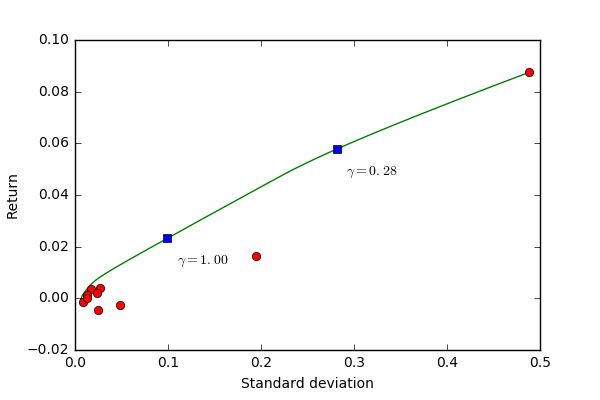
\includegraphics[width=0.8\textwidth]{images/meanvar.png}
\end{figure}

The red dots represent the standard deviation and expected return of the individual stocks. The two blue dots indicate the standard deviation and expected return of the portfolio for two values of $\gamma$. Which value of $\gamma$ we go for depends on how much risk we are willing to take: if we are risk-averse, we may prefer the $\gamma=1$ value to the $\gamma=0.028$ value, at the expense of smaller expected returns.

In practical applications there are a lot of other factors to be considered, such as whether the estimation procedure for the mean and covariance makes sense. In addition, it is often common to add terms that account for \textbf{transaction costs} into the objective funtion.

%\begin{remark}
% There are many problems of interest which are not convex, but in some cases it is possible to formulate an {\em equivalent} convex optimization problem. For example, consider the optimization problem
% \begin{equation}\label{eq:ex1}
%  \minimize x_1^2+x_2^2 \quad \subjto \frac{x_1}{1+x_2^2}\leq 0, \ (x_1+x_2)^2=0.
% \end{equation}
%This problem is not a convex optimization problem (why?). However, the following problem
%\begin{equation}\label{eq:ex2}
% \minimize x_1^2+x_2^2 \quad \subjto x_1\leq 0, \ x_1+x_2=0
%\end{equation}
%is clearly convex, and the solution of~\eqref{eq:ex1} coincides with the solution of~\eqref{eq:ex2}.
%\end{remark}
%
%\section{First order optimality conditions}
%So far we have seen two examples of first order optimality conditions: for unconstraint optimization ($\nabla f(\vct{x})=0$) and for linear programming. We now generalize these to the setting of constrained convex optimization.
%
%\begin{theorem}
% Let $f\colon \R^d\to \R$ be a convex, differentiable function, and 
% \begin{equation*}
%  \mathcal{F}=\{\vct{x} \mid g_i(\vct{x})\leq 0, \ h_j(\vct{x})=0, \ 1\leq i\leq m, \ 1\leq j\leq \ell\}
% \end{equation*}
%a feasible set, with $g_i$ convex and $h_j$ linear. Then $\vct{x}^*$ is an optimal point of the optimization problem
%\begin{equation*}
% \minimize f(\vct{x}) \ \subjto \vct{x}\in \mathcal{F}
%\end{equation*}
%if and only if for all $\vct{y}\in \mathcal{F}$, 
%\begin{equation}\label{eq:opt}
% \ip{\nabla f(\vct{x}^*)}{\vct{y}-\vct{x}^*}\geq 0.
%\end{equation}
%\end{theorem}
%
%\begin{proof}
% Suppose $\vct{x}^*$ is such that~\eqref{eq:constr} holds. Then, since $f$ is a convex function,
% for all $\vct{y}\in \mathcal{F}$ we have, by Theorem 2.4.1,
% \begin{equation*}
%  f(\vct{y})\geq f(\vct{x}^*)+\ip{\nabla f(\vct{x}^*)}{\vct{y}-\vct{x}^*} \geq f(\vct{x}^*),
% \end{equation*}
%which shows that $\vct{x}^*$ is a minimizer in $\mathcal{F}$. To show the opposite direction, assume that $\vct{x}^*$ is a minimizer but that~\eqref{eq:constr} does not hold. This means that there exists a $\vct{y}\in \mathcal{F}$ such that $\ip{\nabla f(\vct{x}^*)}{\vct{y}-\vct{x}^*}<0$. Since both $\vct{x}^*$ and $\vct{y}$ are in $\mathcal{F}$ and $\mathcal{F}$ is convex, any point $\vct{z}(\lambda)=(1-\lambda)\vct{x}^*+t\vct{y}$ with $\lambda\in [0,1]$ is also in $\mathcal{F}$. At $\lambda=0$ we have
%\begin{equation*}
% \frac{df}{d\lambda}f(\vct{z}(\lambda))|_{\lambda=0} = \ip{\nabla f(\vct{x}^*)}{\vct{y}-\vct{x}^*}<0.
%\end{equation*}
%Since the derivative at $\lambda=0$ is negative, the function $f(\vct{z}(\lambda))$ is decreasing at $\lambda=0$, and therefore, for small $\lambda>0$, $f(\vct{z}(\lambda))<f(\vct{z}(0))=f(\vct{x}^*)$, in contradiction to the assumption that $\vct{x}^*$ is a minimizer.
%\end{proof}
%
%\begin{example}
% In the absence of constraints, $\mathcal{F}=\R^d$, and the statement says that
% \begin{equation*}
%  \forall \vct{y}\in \R^d\colon \ip{\nabla f(\vct{x}^*)}{\vct{y}-\vct{x}^*}\geq 0.
% \end{equation*}
%If there was a $\vct{y}$ such that $\ip{\nabla f(\vct{x}^*)}{\vct{y}-\vct{x}^*}>0$, then replacing $\vct{y}$ by $2\vct{x}-\vct{y}$ we also have the converse inequality, and therefore the optimality condition is equivalent to saying that $\nabla f(\vct{x}^*)=\zerovct$. We therefore recover the well-known first order optimality condition from Lecture 2. 
%\end{example}
%
%Geometrically, the first order optimality condition means that the set
%\begin{equation*}
% \{\vct{x}\mid \ip{\nabla f(\vct{x}^*)}{\vct{x}}=\ip{\nabla f(\vct{x}^*)}{\vct{x}^*}\}
%\end{equation*}
%defines a supporting hyperplane to the set $\mathcal{F}$.
%
%\begin{figure}[h!]
%\centering
%\begin{tikzpicture}[thick,rotate=30,scale=0.8]
%\filldraw[color=black, fill=blue!5, very thick](0,0) ellipse (2 and 1.2);
%\node (A1) at (0,-3)  [label=0:{$-\nabla f(\vct{x}^*)$}] {};
%\node (A2) at (0,-1.2)  [label=90:{$\vct{x}^*$}] {};
%%\node (A3) at (0,-2.5)  [label=180:{$\vct{a}$}] {};
%\node (A4) at (-1,0)  [label=180:{$\vct{y}$}] {};
%\filldraw[black] (0,-3) circle (2pt);
%\filldraw[black] (0,-1.2) circle (2pt);
%\filldraw[black] (-1,0) circle (2pt);
%\draw[color=black, thick, <-] (0,-2.9) -- (0,-1.2);
%\draw[color=black, thick, <-] (-0.9,-0.1) -- (0,-1.2);
%\end{tikzpicture}
%\caption{Optimality condition} \label{fig:neg}
%\end{figure}

% %-----------------------------------------------------------------------
% % End of chap1.tex
% %-----------------------------------------------------------------------


%\appendix
%\include{appendix1}

%\backmatter
%\include{biblio}
%\include{index}
\end{document}

%-----------------------------------------------------------------------
% End of chapter.tex
%-----------------------------------------------------------------------
